\documentclass[aspectratio=169,10pt]{beamer}

% ---- THEME ----
\usetheme{Madrid}
\usecolortheme{default}

\definecolor{PrimaryBlue}{HTML}{0B1D3A}
\definecolor{AccentBlue}{HTML}{1C3461}
\definecolor{LightBlue}{HTML}{D6EAF8}
\definecolor{DarkText}{HTML}{1E293B}
\definecolor{MutedGrey}{HTML}{64748B}
\definecolor{RuleGrey}{HTML}{CBD5E1}
\definecolor{CardBG}{HTML}{F7F9FC}
\definecolor{GreenOK}{HTML}{27AE60}
\definecolor{RedWarn}{HTML}{D62728}
\definecolor{AmberNote}{HTML}{E8A838}
\definecolor{TealAccent}{HTML}{16697A}

\setbeamercolor{palette primary}{bg=PrimaryBlue,fg=white}
\setbeamercolor{palette secondary}{bg=AccentBlue,fg=white}
\setbeamercolor{palette tertiary}{bg=PrimaryBlue!80!black,fg=white}
\setbeamercolor{structure}{fg=PrimaryBlue}
\setbeamercolor{title}{fg=white,bg=PrimaryBlue}
\setbeamercolor{frametitle}{fg=white,bg=PrimaryBlue}
\setbeamercolor{block title}{bg=AccentBlue,fg=white}
\setbeamercolor{block body}{bg=LightBlue!40,fg=DarkText}
\setbeamercolor{block title alerted}{bg=RedWarn,fg=white}
\setbeamercolor{block body alerted}{bg=RedWarn!8,fg=DarkText}
\setbeamercolor{block title example}{bg=GreenOK,fg=white}
\setbeamercolor{block body example}{bg=GreenOK!8,fg=DarkText}
\setbeamercolor{item}{fg=AccentBlue}

\setbeamertemplate{navigation symbols}{}
\setbeamertemplate{footline}{%
  \leavevmode\hbox{%
    \begin{beamercolorbox}[wd=.33\paperwidth,ht=2.5ex,dp=1ex,left]{palette primary}%
      \hspace*{2ex}\tiny\insertshortauthor
    \end{beamercolorbox}%
    \begin{beamercolorbox}[wd=.34\paperwidth,ht=2.5ex,dp=1ex,center]{palette primary}%
      \tiny\insertshorttitle
    \end{beamercolorbox}%
    \begin{beamercolorbox}[wd=.33\paperwidth,ht=2.5ex,dp=1ex,right]{palette primary}%
      \tiny\insertframenumber\,/\,\inserttotalframenumber\hspace*{2ex}
    \end{beamercolorbox}%
  }%
}

\addtobeamertemplate{block begin}{}{\vspace{-3pt}}
\addtobeamertemplate{block end}{\vspace{-4pt}}{}

% ---- PACKAGES ----
\usepackage{hyperref} % Add this in your preamble
\usepackage{amsmath,amssymb}
\usepackage{graphicx}
\usepackage{booktabs}
\usepackage{tikz}
\usetikzlibrary{arrows.meta,positioning,calc,shadows.blur}
\usepackage{hyperref}
\usepackage{array}
\usepackage{colortbl}
\usepackage{pifont}
\usepackage[most]{tcolorbox}

\newcommand{\cmark}{\textcolor{GreenOK}{\ding{51}}}
\newcommand{\xmark}{\textcolor{RedWarn}{\ding{55}}}

\newcommand{\tightmath}{%
  \setlength{\abovedisplayskip}{0pt}%
  \setlength{\belowdisplayskip}{0pt}%
  \setlength{\abovedisplayshortskip}{0pt}%
  \setlength{\belowdisplayshortskip}{0pt}%
}

% ---- Chipcard: numbered card with colored left stripe ----
\newcommand{\chipcard}[4]{%
  \begin{tcolorbox}[
    enhanced, colback=white, colframe=RuleGrey, boxrule=0.4pt, arc=1pt,
    left=7pt,right=5pt,top=4pt,bottom=3pt,
    borderline west={3pt}{0pt}{#1},
    drop shadow={black!25,yshift=-0.8pt}
  ]
  {\tikz[baseline=(X.base)]\node[circle,fill=#1,text=white,inner sep=1pt,
        minimum size=12pt,font=\tiny\bfseries] (X) {#2};}%
  \hspace{2pt}{\color{#1}\bfseries\small #3}\\[0.5pt]
  \scriptsize #4
  \end{tcolorbox}%
}

% ---- Stripe-only card (no number chip) ----
\newcommand{\stripecard}[3]{%
  \begin{tcolorbox}[
    enhanced, colback=white, colframe=RuleGrey, boxrule=0.4pt, arc=1pt,
    left=7pt,right=7pt,top=4pt,bottom=3pt,
    borderline west={3pt}{0pt}{#1},
    drop shadow={black!25,yshift=-0.8pt}
  ]
  {\color{#1}\bfseries\small #2}\\[1pt]
  \scriptsize #3
  \end{tcolorbox}%
}

% ---- Reference card: number chip + category label + citation ----
\newcommand{\refcard}[4]{%
  % #1 accent color, #2 ref number, #3 category label, #4 citation body
  \begin{tcolorbox}[
    enhanced, colback=white, colframe=RuleGrey, boxrule=0.4pt, arc=1pt,
    left=7pt,right=7pt,top=3pt,bottom=3pt,
    borderline west={3pt}{0pt}{#1},
    drop shadow={black!25,yshift=-0.8pt}
  ]
  {\tikz[baseline=(X.base)]\node[circle,fill=#1,text=white,inner sep=1pt,
        minimum size=13pt,font=\scriptsize\bfseries] (X) {#2};}%
  \hspace{3pt}{\color{#1}\bfseries\footnotesize #3}\\[1pt]
  \scriptsize #4
  \end{tcolorbox}%
}

% ---- META ----
\title[Efficient IM-FHSS]{Efficient Index Modulation Based FHSS}
\subtitle{A Unified Anti-Jamming Perspective}
\author[C. Arjun \& P. Tiwari]{C. Arjun \and Prashant Tiwari}
\institute[]{Based on Shi \textit{et al.}, IEEE TVT}
\date{Academic Year 2025-26}

\begin{document}

% ========== SLIDE 1: TITLE ==========
\begin{frame}[plain]
\vfill
\begin{center}
{\color{PrimaryBlue}\rule{0.9\textwidth}{1.2pt}}\\[10pt]
{\LARGE\bfseries\color{PrimaryBlue} Signal Propagation in Transformers }\\[4pt]
{\Large\bfseries\color{PrimaryBlue} Stable-rank analysis and web app for Vision and Text Transformer}\\[8pt]
{\Large\bfseries\color{PrimaryRed} Guide : Prof. Sumantra Dutta Roy}\\[8pt]

{\color{PrimaryBlue}\rule{0.9\textwidth}{1.2pt}}\\[14pt]
\end{center}


\begin{block}{\small Simranjit Singh [2025EEE2834]}
\scriptsize
\textit{Contributions}
\begin{itemize}\setlength\itemsep{2pt}\setlength\topsep{2pt}
  \item Literature survey
  \item Gap identification and Signal Propagation theories. 
  \item Stable rank simulation across all experiments
\end{itemize}
\end{block}


\vspace{6pt}
\begin{center}
{\small\color{DarkText!70} MTech Communication Engineering \& Computer Technology \quad $\bullet$ \quad Academic Year 2025--26}
\end{center}
\vfill
\end{frame}


% ========== SLIDE 2: TIMELINES, RESEARCH GAP & SYSTEM MODEL ==========
\begin{frame}[plain]
\vspace{1pt}

\hspace{6pt}{\Large\bfseries\color{PrimaryBlue} Timelines, Research Gap \& System Model}%
\hfill{\footnotesize\itshape\color{MutedGrey}}\hspace{6pt}\\[-3pt]
\hspace{6pt}{\color{RedWarn}\rule{1.1cm}{1.6pt}}\\[4pt]

% --- ROW 1: full-width figure banner ---
\hspace{6pt}%
\begin{minipage}{\dimexpr\textwidth-12pt\relax}
\begin{tcolorbox}[
  enhanced, colback=white, colframe=RuleGrey, boxrule=0.4pt, arc=1pt,
  height=3.7cm, valign=center,
  left=4pt,right=4pt,top=2pt,bottom=2pt
]
\centering\includegraphics[height=3.3cm,keepaspectratio]{time1.png}
\end{tcolorbox}
\end{minipage}

\vspace{4pt}

% --- ROW 2: two content blocks side-by-side (original content, verbatim) ---
\begin{columns}[T,onlytextwidth]

\begin{column}{0.495\textwidth}
\tightmath
\stripecard{RedWarn}{Research Gap}{%
Prior works such as \textit{Mind the Gap} and \textit{Differential Attention} primarily focus on architectural or robustness improvements, but lack a \textbf{rigorous spectral analysis of Transformer representations}. No systematic studies examine how \textbf{information propagation and stability evolve across layers} in terms of singular value distributions/effective dimensionality. While \textit{Differential Attention} improves training stability heuristically, it does not quantify stability using principled metrics, nor does it analyze how attention and feed-forward blocks impact the \textbf{collapse or preservation of feature subspaces}. Furthermore, there is no unified analysis across modalities.
}

\end{column}

\begin{column}{0.495\textwidth}
\tightmath
\stripecard{AccentBlue}{Stable Rank ($\rho$)}{%
{\color{AccentBlue}\bfseries Concept:} It quantifies the \emph{effective dimensionality} of a matrix $W$ by measuring the distribution of its SV spectrum $\{\sigma_1, \sigma_2, \dots, \sigma_r\}$. 
\begin{equation*}
    \rho(W) = \frac{\|W\|_F^2}{\|W\|_2^2} = \frac{\sum_{i=1}^{r} \sigma_i^2}{\sigma_{\max}^2}
\end{equation*}
% where $\|W\|_F$ is the Frobenius norm and $\|W\|_2 = \sigma_{\max}$ is the spectral norm.

\begin{itemize}
    \item {Balanced Spectrum:} $\rho(W) \to \text{rank}(W) \implies$ High-dimensional information flow.
    \item {Dominant Mode:} $\rho(W) \to 1 \implies$ Representation collapse/singularity.
\end{itemize}

}
\end{column}

\end{columns}
\end{frame}


% ========== SLIDE 3: CORE TECHNICAL & MATHEMATICAL DETAILS ==========
\begin{frame}[plain]
\vspace{1pt}
\hspace{6pt}{\Large\bfseries\color{PrimaryBlue} Technical \& Mathematical framework}%
\hfill{\footnotesize\itshape\color{MutedGrey} }\hspace{6pt}\\[-3pt]
\hspace{6pt}{\color{RedWarn}\rule{1.1cm}{1.6pt}}\\[2pt]

\tightmath

\begin{columns}[T,onlytextwidth]

\begin{column}{0.495\textwidth}

\chipcard{AccentBlue}{1}{Encoder-Decoder Architecture}{%
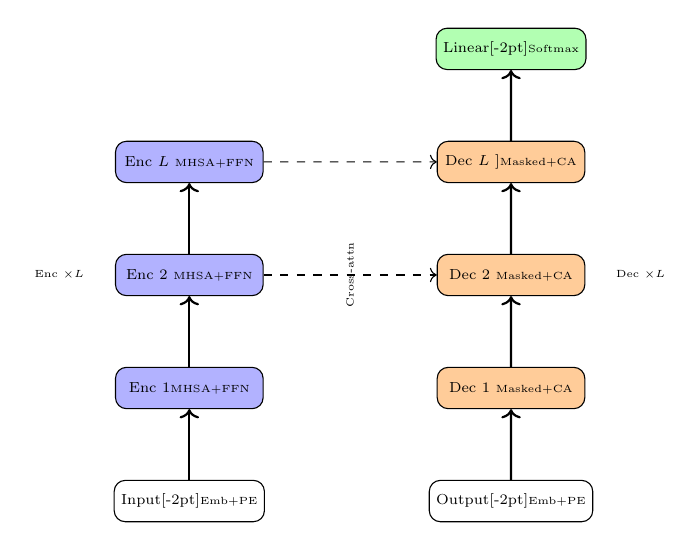
\begin{tikzpicture}[
scale=0.75,
every node/.style={scale=0.75},
node distance=0.9cm and 1.2cm,
block/.style={draw, rounded corners, minimum width=2.5cm, minimum height=0.7cm, align=center},
arrow/.style={->, thick}
]

% -------- Encoder --------
\node[block, fill=blue!30] (enc1) {\scriptsize Enc 1\tiny MHSA+FFN};
\node[block, fill=blue!30, above=of enc1] (enc2) {\scriptsize Enc 2 \tiny MHSA+FFN};
\node[block, fill=blue!30, above=of enc2] (encL) {\scriptsize Enc $L$ \tiny MHSA+FFN};

\node[block, below=of enc1] (embed) {\scriptsize Input[-2pt]\tiny Emb+PE};

\draw[arrow] (embed) -- (enc1);
\draw[arrow] (enc1) -- (enc2);
\draw[arrow] (enc2) -- (encL);

\node[left=0.3cm of enc2] {\tiny Enc $\times L$};

% -------- Decoder --------
\node[block, fill=orange!40, right=2.2cm of enc1] (dec1) {\scriptsize Dec 1 \tiny Masked+CA};
\node[block, fill=orange!40, above=of dec1] (dec2) {\scriptsize Dec 2 \tiny Masked+CA};
\node[block, fill=orange!40, above=of dec2] (decL) {\scriptsize Dec $L$ ]\tiny Masked+CA};

\node[block, below=of dec1] (outembed) {\scriptsize Output[-2pt]\tiny Emb+PE};

\draw[arrow] (outembed) -- (dec1);
\draw[arrow] (dec1) -- (dec2);
\draw[arrow] (dec2) -- (decL);

\node[right=0.3cm of dec2] {\tiny Dec $\times L$};

% -------- Output --------
\node[block, fill=green!30, above=of decL] (softmax) {\scriptsize Linear[-2pt]\tiny Softmax};
\draw[arrow] (decL) -- (softmax);

% -------- Cross Attention --------
\draw[->, dashed] (encL.east) -- (decL.west);
\draw[->, dashed] (enc2.east) -- (dec2.west);

\node[rotate=90] at ($(enc2)!0.5!(dec2)$) {\tiny Cross-attn};

\end{tikzpicture}
}





\vspace{3pt}




\end{column}

\begin{column}{0.495\textwidth}

\chipcard{AmberNote}{2}{LayerNorm & Residuals}{%
{\color{AmberNote}\bfseries Residual Connection:}
[
\mathbf{H}' = \mathbf{H} + \mathcal{F}(\mathbf{H})
]
{\color{MutedGrey}\tiny\itshape $\mathcal{F}$: sublayer (Attention / FFN). Enables identity mapping and gradient flow.}

{\color{AmberNote}\bfseries Layer Normalization:}
[
\mathrm{LayerNorm}(\mathbf{h}) = \frac{\mathbf{h} - \mu}{\sqrt{\sigma^2 + \epsilon}} \cdot \gamma + \beta
]
{\color{MutedGrey}\tiny\itshape $\mu,\sigma^2$: mean/variance across features; $\gamma,\beta$: learnable scale/shift.}

{\color{AmberNote}\bfseries Effect:}
[
|\mathbf{J}| \approx 1 ;\Rightarrow; \text{stable gradients, controlled activations}
]

{\color{PrimaryBlue}\bfseries\scriptsize Role:; prevents vanishing/exploding gradients, stabilizes training, preserves information flow across deep Transformer layers.}%
}

\vspace{3pt}

\chipcard{RedWarn}{3}{Differential \& MTG Attention}{%
{\color{RedWarn}\bfseries 1st:} 
Captures \textit{relative feature change} via mean-normalization:
\begin{equation*}
    \text{Attn}_{\Delta} = \text{softmax} \left( \frac{(Q-\bar{Q})(K-\bar{K})^\top}{\sqrt{d}} \right) V
\end{equation*}
{\color{MutedGrey}\tiny $\bar{Q},\bar{K}$ denote mean-normalized tensors; suppresses dominant noise modes.}

\vspace{2pt}
{\color{RedWarn}\bfseries 2nd:} 
Penalizes the dominance of the leading singular value $\sigma_1$:
\begin{equation*}
    \Delta_\sigma = \sigma_1 - \sigma_2 \implies \text{Attn}_{\text{MTG}} = \text{softmax} \left( \frac{QK^\top}{\sqrt{d}} - \lambda \Delta_\sigma \right) V
\end{equation*}
{\color{MutedGrey}\tiny Penalizing $\Delta_\sigma$ reduces spectral gap $\Rightarrow$ prevents rank collapse.}
%
}
\end{column}
\end{columns}
\end{frame}


% ========== SLIDE 4: PLOTS & INTERPRETATIONS ==========
\begin{frame}[plain]
\vspace{-2pt}

\hspace{6pt}{\Large\bfseries\color{PrimaryBlue} Plots and Results}%
\hfill{\footnotesize\itshape\color{MutedGrey} }\hspace{6pt}\\[-3pt]
\hspace{6pt}{\color{RedWarn}\rule{1.1cm}{1.6pt}}\\[3pt]

\begin{columns}[T,onlytextwidth]

\begin{column}{0.49\textwidth}

\centering

\includegraphics[width=0.82\textwidth,height=0.24\textheight,keepaspectratio]{plot1.png}\\[-2pt]
{\scriptsize\textbf{(a) Vanilla Transformer} (No LayerNorm $+$ No Residuals)}\\[-3pt]
{\tiny\itshape SR $\approx$ 1.03\,---\,All layers converge to near rank-1, confirming severe representation collapse. Without normalization or skip connections, attention weights degenerate into rank-deficient projections, crippling gradient flow.}

\vspace{0pt}


\includegraphics[width=0.82\textwidth,height=0.24\textheight,keepaspectratio]{plot3.png}\\[-2pt]
{\scriptsize\textbf{(c) Differential Transformer} (RMSNorm $+$ SwiGLU FFN)}\\[-3pt]
{\tiny\itshape SR $\approx$ 1.48\,---\,Dual-branch attention with $\lambda$-scaled subtraction actively suppresses noisy attention patterns, yielding markedly higher effective rank. SwiGLU gating and RMSNorm further stabilize spectral dynamics across depth.}

\end{column}

\begin{column}{0.49\textwidth}

\centering

\includegraphics[width=0.82\textwidth,height=0.24\textheight,keepaspectratio]{plot2.png}\\[-2pt]
{\scriptsize\textbf{(b) Residual Transformer} (Pre-LayerNorm $+$ Residuals)}\\[-3pt]
{\tiny\itshape SR $\approx$ 1.28\,---\,Residual shortcuts partially restore gradient pathways and Pre-LayerNorm reduces internal covariate shift, lifting SR above baseline. However, moderate rank deficiency persists in deeper layers.}

\vspace{0pt}


\includegraphics[width=0.82\textwidth,height=0.24\textheight,keepaspectratio]{plot4.png}\\[-2pt]
{\scriptsize\textbf{ \hspace{1em} (d) Mind The Gap Transformer}\newline (Score-centering \& variance-normalized $+$ residuals)}\\[-3pt]
{\tiny\itshape SR $\approx$ 1.51\,---\,Score-centering removes the mean bias from attention logits while variance normalization controls spread, achieving the highest and most uniform SR across all layers\,---\,indicating optimal signal propagation health.}

\end{column}

\end{columns}

\end{frame}



% ========== SLIDE 5: RESULTS & NOVELTY ==========
\begin{frame}[plain]
\vspace{2pt}

\hspace{6pt}{\large\bfseries\color{PrimaryBlue} Results and Novelty: Live SVD Diagnostics}%
\hfill{\tiny\itshape\color{MutedGrey} \href{http://35.223.97.175:3000/}{Transformer Dashboard}}\hspace{6pt}\\[-3pt]
\hspace{6pt}{\color{RedWarn}\rule{1.1cm}{1.6pt}}\\[2pt]

\begin{columns}[t]
\begin{column}{0.56\textwidth}
    {\footnotesize\textbf{Key Empirical Findings}}
    \vspace{-3pt}
    \begin{itemize}\setlength\itemsep{-1pt}\setlength\parskip{0pt}
        \item[\tiny$\bullet$] {\tiny\textbf{Monotonic SR Ordering:} Across both CIFAR-10 and AG News, stable rank follows a strict hierarchy: Vanilla\,(1.03) $<$ Residual\,(1.28) $<$ Differential\,(1.48) $<$ MtG\,(1.51) --- confirming SR as a \textbf{domain-agnostic} diagnostic.}
        \item[\tiny$\bullet$] {\tiny\textbf{Rank-1 Collapse Confirmed:} Without normalization or skip connections, all layers converge to $SR \approx 1.0$, empirically validating theoretical predictions of representation collapse.}
        \item[\tiny$\bullet$] {\tiny\textbf{Depth-Dependent Diversity:} In Residual Transformer, deeper layers maintain \textit{higher} SR ($SR_{L5} > SR_{L0}$), suggesting residual shortcuts create gradient highways that preferentially benefit deeper representations.}
        \item[\tiny$\bullet$] {\tiny\textbf{Cross-Domain Generalization:} Identical SR ordering holds for both Vision (CIFAR-10, ViT) and Text (AG News, Encoder) --- the diagnostic transfers without task-specific tuning.}
    \end{itemize}

    \vspace{-1 pt}
    {\footnotesize\textbf{Novel Contributions}}
    \vspace{-4pt}
    \begin{itemize}\setlength\itemsep{-1pt}\setlength\parskip{0pt}
        \item[\tiny$\bullet$] {\tiny\textbf{Gap:} No standard framework (PyTorch / HuggingFace / JAX) computes Stable Rank natively during training.}
        \item[\tiny$\bullet$] {\tiny\textbf{Solution:} Non-blocking CPU-offloaded SVD subset sampling every 50 steps --- zero GPU overhead, continuous monitoring.}
        \item[\tiny$\bullet$] {\tiny\textbf{} \textbf{Stable Rank} unifies transformer diagnostics across architectures and domains --- a single scalar that captures what loss curves, gradient norms, and  attention entropy cannot: the \textit{effective dimensionality} of learned representations at each layer.}
    \end{itemize}
\end{column}

\begin{column}{0.42\textwidth}
    \refcard{RedWarn}{1}{Rank Collapse Detection}{%
    Vanilla SR $\approx 1.0$ across all 6 layers --- attention weights collapse to rank-deficient projections; training accuracy plateaus at $\sim$52\%.%
    }
    \vspace{0pt}
    \refcard{TealAccent}{2}{SR as Early-Stop Signal}{%
    When SR/Steps curve plateaus while val-loss rises, it indicates memorization onset --- enabling \textbf{automated overfitting detection} without holdout sets.%
    }
    \vspace{0pt}
    \refcard{AmberNote}{3}{Implementation}{%
    $SR(W) = \frac{\sum \sigma_i^2}{\sigma_{\max}^2}$\,; computed via \texttt{torch.linalg.svdvals} on CPU-detached weights to avoid GPU synchronization stalls.%
    }
\end{column}
\end{columns}

\vspace{-2 pt}

\end{frame}


\end{document}